\documentclass[11pt]{report}
\usepackage{graphicx}
\usepackage{float}
\title{EE314 Experiment 5 Flip-Flops and Sequential Circuits}
\date{2018\\ April}
\author{Nail Tosun - 2094563\\ Electric and Electronic Engineering Departmant, METU}
\begin{document}
\maketitle
1)
\begin{figure}[H]
  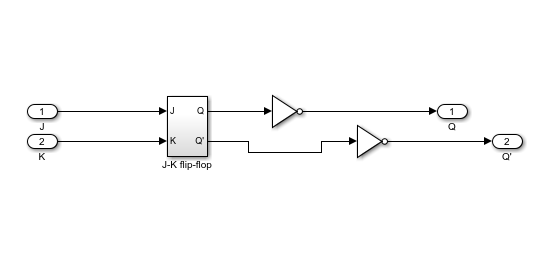
\includegraphics[width=\linewidth]{1}
  \caption{Logic design for Question 1}
  \label{fig:zero}
\end{figure}
2)\[Q_{1n}=JQ'_{1n-1}+K'Q_{1n-1}\]
\[J=Q'_{3n-1}Q'_{2n-1} \>\>\> K=Q_{3n-1}Q_{2n-1} \]
\[K'=Q'_{3n-1}+Q'_{2n-1}\]
\[Q_{1n}=Q'_{3n-1}Q'_{2n-1}Q'_{1n-1}+(Q'_{3n-1}+Q'_{2n-1})Q_{1n-1}\]
\[Q_{2n}=JQ'_{2n-1}+K'Q_{2n-1}\]
\[J=Q_{1n} \>\>\> K'=Q_{1n}\]
\[Q_{2n}=Q_{1n}Q'_{2n-1}+Q_{1n}Q_{2n-1}\]
\[Q_{2n}=2Q_{3n-1}Q'_{2n-1}Q'_{1n-1}+Q'_{2n-1}Q_{1n-1}+Q_{2n-1}Q_{1n-1}Q'_{3n-1}\]
\[Q_{3n}=JQ_{3n-1}+KQ'_{3n-1}\]
\[J=Q_{2n} \>\>\> K=Q_{2n}\]
\[Q_{3n}=2Q_{3n-1}Q'_{2n-1}Q'_{1n-1}+Q_{3n-1}Q'_{2n-1}Q_{1n-1}\]
3)
\begin{figure}[H]
  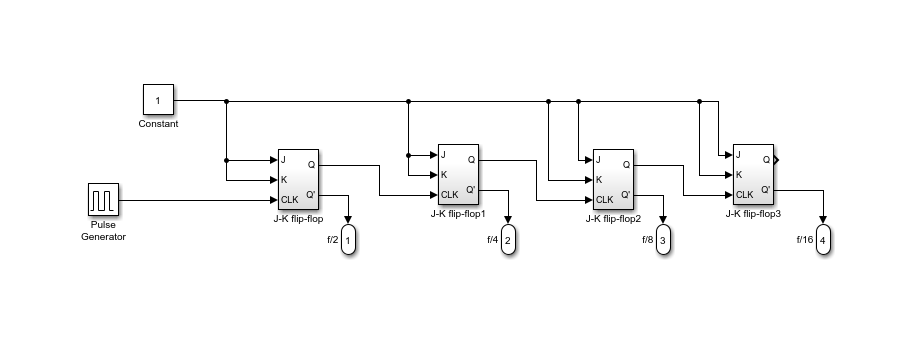
\includegraphics[width=\linewidth]{frequecy}
  \caption{Frequency Converter Logic Design}
  \label{fig:zero}
\end{figure}
4)
\begin{figure}[H]
  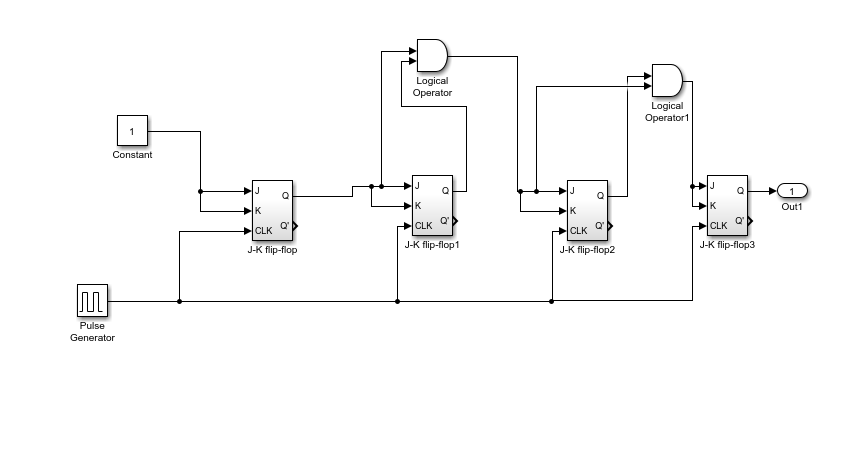
\includegraphics[width=\linewidth]{upcounter}
  \caption{Ripple Up Counter}
  \label{fig:zero}
\end{figure}
5)
\begin{figure}[H]
  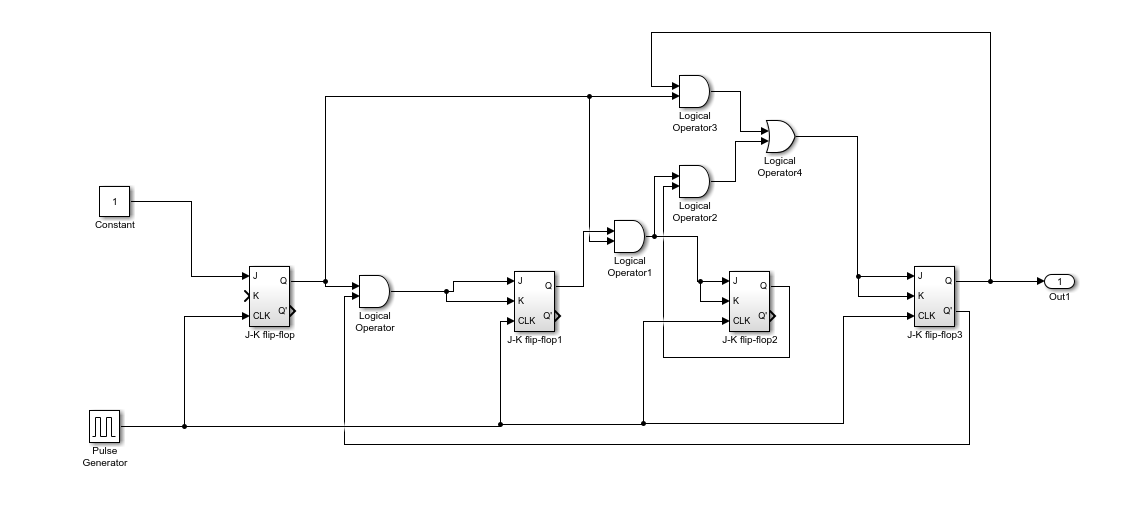
\includegraphics[width=\linewidth]{five}
  \caption{BCD counter}
  \label{fig:zero}
\end{figure}
6)
\begin{figure}[H]
  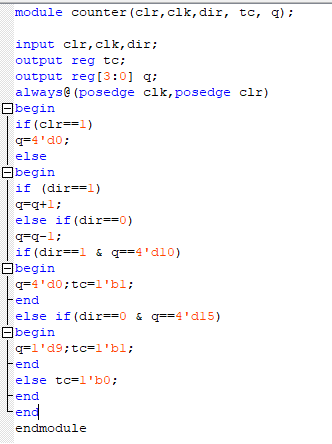
\includegraphics[scale=0.7]{v}
  \caption{Verilog Code}
  \label{fig:zero}
\end{figure}

\begin{figure}[H]
  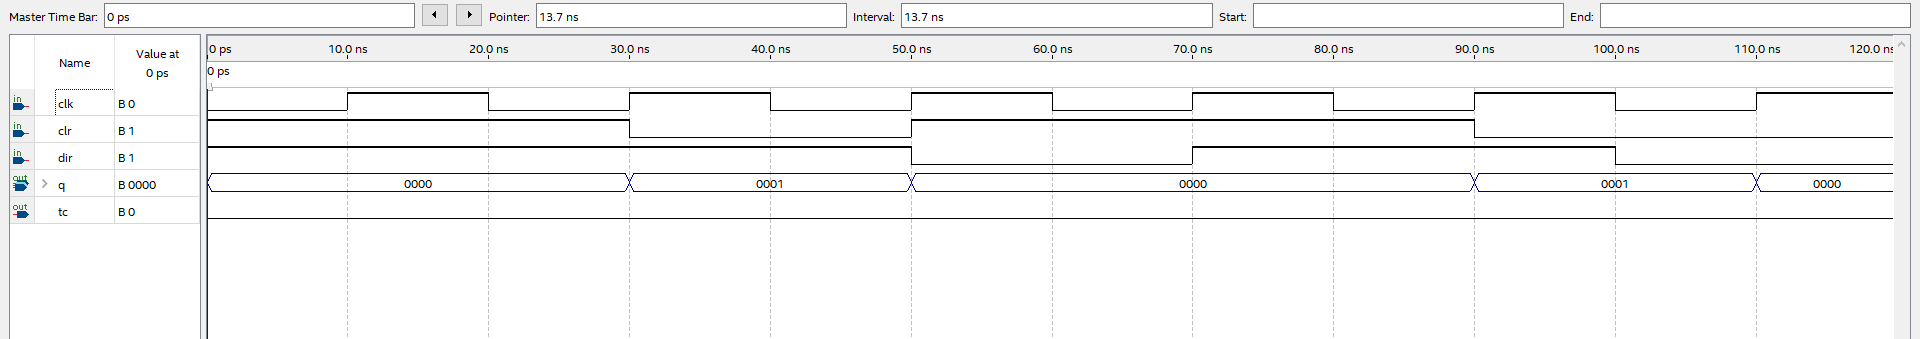
\includegraphics[width=\linewidth]{cooonter1}
  \caption{BCD counter Simulation results}
  \label{fig:zero}
\end{figure}
\end{document}